\documentclass{beamer}
\usepackage{mathtools, amsmath, xcolor, graphicx}
\usetheme{Rochester}
\usecolortheme{dolphin}

\author{Joe Bentley and Jake Lane}

\title{Higgs Signal Optimisation}

\institute{}
\subject{Physics}
\date{}
\begin{document}


\frame{\titlepage}


\frame{
\frametitle{Summary}
\begin{enumerate}
\item Kinematic variables
\item Background
\item How Higgs signals are simulated
\item How the signals are interpreted
\item How the Higgs signal is optimised
\item Possible expansions of the project
\end{enumerate}
}

\frame{
\frametitle{Kinematic Variables}
4-momentum, $p^{\mu}$ is defined by 3 parameters for a photon:
\begin{align}
E = p^t &= p_T \cosh{\eta} \\
p^x &= p_T \cos{\phi}\\
p^y &= p_T \sin{\phi}\\
p^z &= p_T \sinh{\eta}
\end{align}
\begin{enumerate}
  \item $p_T$ is the transverse momentum (the component of momentum perpendicular to the beam axis)
\item $\eta$ is the pseudo rapidity (which is the rapidity for a photon)
\item $\phi$ is the azimuthal angle
\end{enumerate}

}

\frame{
\frametitle{Kinematic Variables}
\begin{itemize}
\item $\Delta \phi$ is Lorentz invariant since the angle is measured in a plane perpendicular to the beam line (subject to Lorentz transformations)
\end{itemize}
}

\frame{
  \frametitle{Kinematic Variables}
  Photons have the property $E = p = \sqrt{(p^x)^2 + (p^y)^2 + (p^z)^2}$ so rapidity $y$ is the same as the pseudo rapidity, $\eta$.
  \begin{align*}
  \eta &\equiv \frac{1}{2} \log(\frac{p +p^z}{p - p^z}) \\
  	&= \frac{1}{2} \log(\frac{E + p^z}{E - p^z}) \equiv y
 \end{align*}
  \begin{enumerate}
  \item Rapidity allows for a measure of how far forwards the photon travels parallel to the beam line
  \item The differences $\Delta \phi^2$ and $\Delta \eta^2$ are Lorentz invariant so we can use these instead of a polar angle in the photon frame.
  \end{enumerate}
}


\frame{
\frametitle{Background}
The Higgs boson is produced in many channels.
The most common in proton collider experiments is 'gluon gluon Fusion' (ggF)
\pause
\begin{figure}
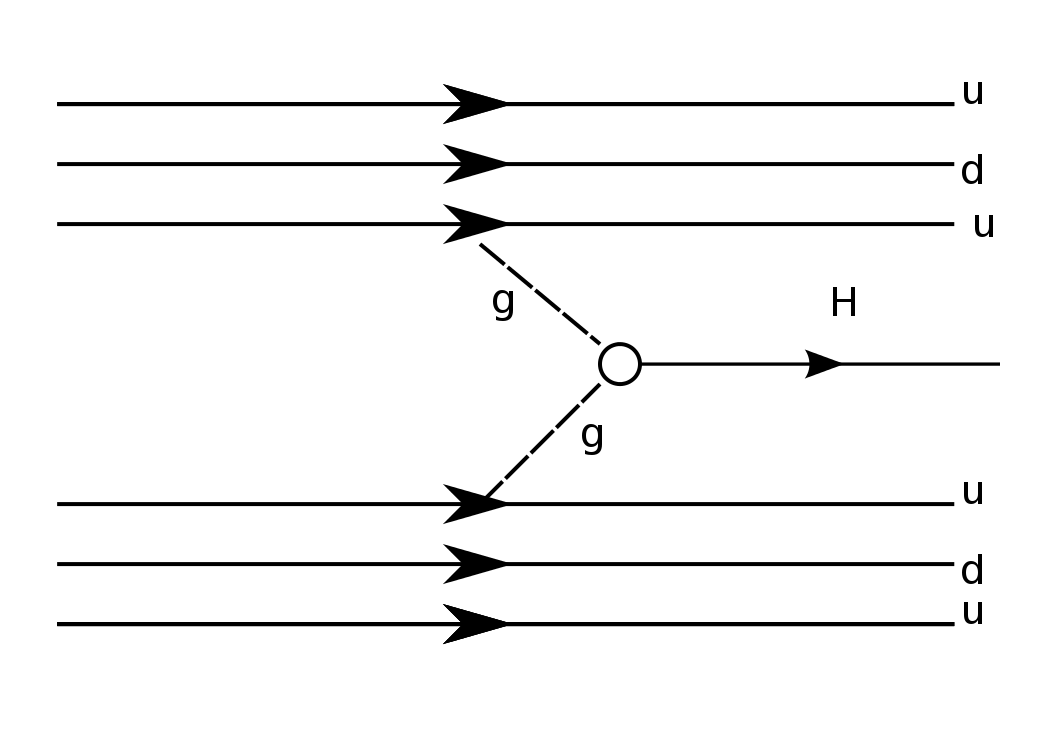
\includegraphics[scale = 0.15]{VBF.png}
\caption{Gluons fusing into a Higgs at a proton-proton interaction, note the circle at the meeting of the 2 gluons represents the various quark (or W boson) loops that produce the Higgs}
\end{figure}
}

\frame{
\frametitle{Decay}
The Higgs decays in a very short period of time in many channels, the most common is 2 bottom quarks, but we investigate the decay into 2 photons (the diphoton channel.)
\begin{figure}
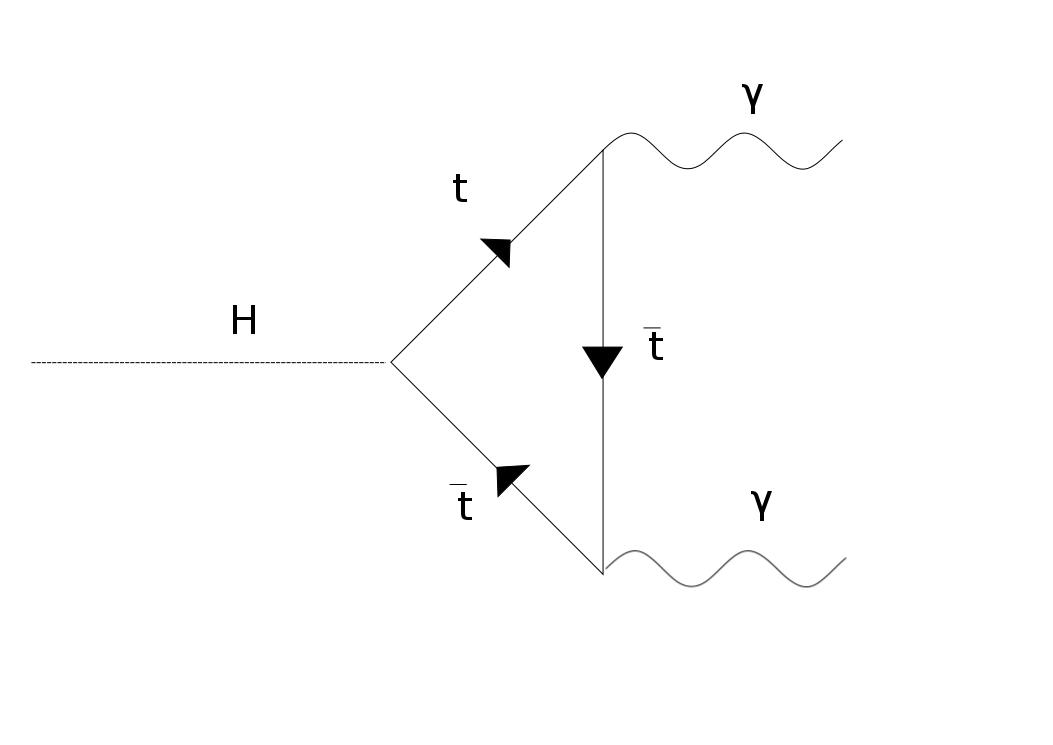
\includegraphics[scale=0.13]{Hyy.png}
\caption{Decay of Higgs into 2 photons}
\end{figure}
}


\frame{
\frametitle{Simulation}

\begin{itemize}
  \item The Higgs events and background events provided to us are simulated using PYTHIA.
  \item The simulation consists of a text file of the Energy and momentum (four momentum) of each photon in each collision event
  \item We will use one simulation of 10,000 Higgs events and one simulation of 1,000,000 background events
\end{itemize}

}

\frame{
\frametitle{Parsing}

\begin{itemize}
  \item To parse the events, we wrote a script in Python 3 to parse the four momenta from the event data
  \item It calculates the invariant mass of each decay event and outputs this to a plaintext file for plotting in a histogram
  \item It can also apply a range of filtering on the events to filter out events that are not Higgs
  \item The script is written as a module so that we can use it from other scripts, for example we use it in the statistical significance script to apply the filtering
\end{itemize}
}


\frame{
\frametitle{Weighting}

\begin{itemize}
  \item In our simulated data, there are 10,000 Higgs events, and 1,000,000 background events. In an actual collider experiment this ratio would be much lower
  \item To account for this we need to apply weightings to each dataset, to make the Higgs less prominent or the background more prominent
  \item We can apply the weightings directly when calculating our histogram
\end{itemize}

\pause

\begin{align*}
  \frac{\text{num. Higgs events}}{\text{num. background events}} = \frac{\sigma{\left(\text{Higgs produced}\right)} \times B_f\left(H\to\gamma\gamma\right)}{\sigma{\left(\text{background}\right)}}
\end{align*}
}

\frame{
\frametitle{Weighting}
\begin{itemize}
\item Higgs signals are weighted to produce a probability of producing a Higgs and that the Higgs decays into 2 photons and taking the ratio of simply producing 2 background photons
\item The weighting is constructed such that the background events have weightings of 1
\end{itemize}
}

\frame{
\frametitle{Filtering}

\begin{itemize}
  \item There are $\sim$ 100 Higgs events to $\sim$ 100,000,000 background events
  \item If we do not have good filtering then there is no chance of seeing the Higgs events amongst the background events
  \item We need an effective way to distinguish Higgs events from background events
\end{itemize}
}

\frame{
  \frametitle{Filter Methods}

  \begin{enumerate}
    \item Number of particles
    \item Transverse momentum
    \item Energy
    \item Azimuthal angle
  \end{enumerate}
}

\frame{
  \frametitle{Filter Methods}
\begin{enumerate}
\item Number cut so that only events with 2 or more photons are counted
\item 2 Transverse momentum, $p_T$, cuts so that 1 photon has a larger $p_T$ than $p_{T1}$ and the other has a $p_T > p_{T2}$
\item 2 Energy $E$ cuts, in a similar principle to the $p_T$ cuts
\item Cuts for the angular difference between the 2 photons derived from the difference in azimuthal angle $\Delta \phi^2$ and the difference in pseudorapidity, $\Delta \eta^2$
\end{enumerate}
}

\frame{
\frametitle{Physical meaning behind filtering}
\begin{itemize}
\item $E$ make the assumption that photons in the Higgs decay will be of high energy (or momentum)
\item Transverse cuts which allow for photons to be cut that mainly decay perpendicular to the beam line.
\item The $\Delta \eta$ and $\Delta \phi$ cuts allow for a Lorentz invariant angular separation between the photons. We can construct events that are 'back to back' which we expect from a Higgs decaying.
\end{itemize}
}

\frame{
\frametitle{Optimising our Filters}

To optimise our filters so that we have the best ratio of Higgs events to background events, we need to optimise our filter methods for the highest statistical significance $\Sigma$,

\begin{equation}
\Sigma \equiv \frac{S}{\sqrt{S + B}}
\end{equation}

where $S$ is the number of filtered signal events and $B$ is the number of filtered background events.

\pause

We apply the filtering and calculate the significance for a series of different parameters, for example for different transverse momenta cuts, to see what gives us the best statistical significance.
}

\frame{
\frametitle{Optimising our Filters}

\begin{figure}
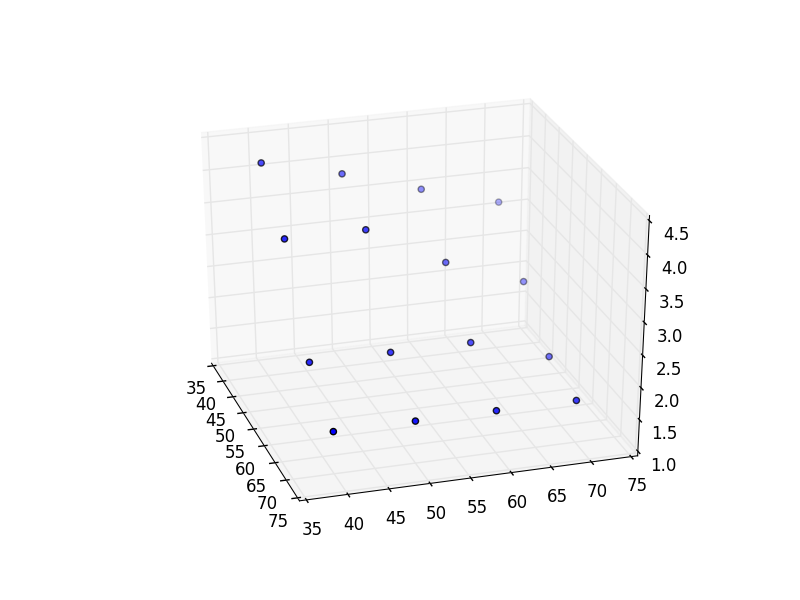
\includegraphics[scale=0.2]{significance1}
\caption{Statistical significance (height of points) for a series of different transverse momenta}
\end{figure}

This is a 3D plot generated from a script that calculates the statistical signifiance for various transverse momenta cuts. From graphs like these we can narrow down the ranges of transverse momenta that we filter until we get the highest statistical significance. We use PyPlot (matplotlib) to generate our plots.
}

\frame{
  We can use the same method to check for example which azimuthal angles gives the highest statistical significance, by plotting a 2D scatter graph of statistical significance against scatter angle.
}


\frame{
\frametitle{Invariant mass histogram}

We calculate a histogram of invariant mass of the diphoton system ($m_{\gamma \gamma}$) using the 'numpy' (numerical python) library.
Whilst this is not the primary aim (optimising a signal) it gives a visual representation of signal strength (i.e. 'seeing the Higgs').

}

\frame{
\frametitle{Issues}

\begin{itemize}
  \item Since there are were so many background events, the python script was slow. Fixed by using script to generate four momentum count headers on each event. This allowed us to pre-calculate how many four momenta are in a given event, which is much faster.
\end{itemize}

}

\frame{
\frametitle{Further Explorations}

Could possibly observe a different decay channel. Jets. Experimentation with PYTHIA.

\begin{itemize}
  \item Since we have access to PYTHIA, the program that simulated the data, we could potentially generate new data
  \item Since our program is quite general, it wouldn't be too difficult to alter it for other Higgs decays
  \item The program being entered around photon data would require changes to the filtering as we would have 4 momenta with non-zero invariant masses, so that background simulation is much more difficult, involving different particles.
\end{itemize}

}


\frame{
\frametitle{Conclusion/Questions}



Any questions?
}

\end{document}
